% Fuente: Auxiliar 8, «Árbol de Branch and Bound».
Suponga que para 
\[
\max \{c^T x : Ax = b, x \geq 0, x \in \mathbb{Z}^n \}
\]
se obtiene el árbol de Branch and Bound de la Figura~\ref{ex:5:1:fig:arbol}. Responda las siguientes preguntas:

\begin{enumerate}
    \item Si ejecutamos B\&B con un \textit{gap} relativo de 10\% y una cota inferior inicial de $-\infty$, ¿es posible terminar después de explorar sólo cuatro nodos? Si es así, ¿cuáles serían las hojas sin explorar?
    \item Si ejecutamos B\&B, y exploramos el nodo 4 antes del nodo 7, ¿sería posible que el nodo 12 sea explorado en algún momento posterior por el algoritmo? Justifique.
    \item Usando sólo el árbol mostrado en la figura, ¿es posible encontrar la solución óptima del problema? Justifique.
    \item ¿Es posible que el conjunto de nodos \textbf{5, 10, 11, 7} sean las hojas del algoritmo de B\&B? Justifique.
    \item ¿Es posible que el conjunto de nodos \textbf{2, 6, 12, 13} sean las hojas del algoritmo de B\&B? Justifique.
\end{enumerate}

\begin{figure}
    \centering
    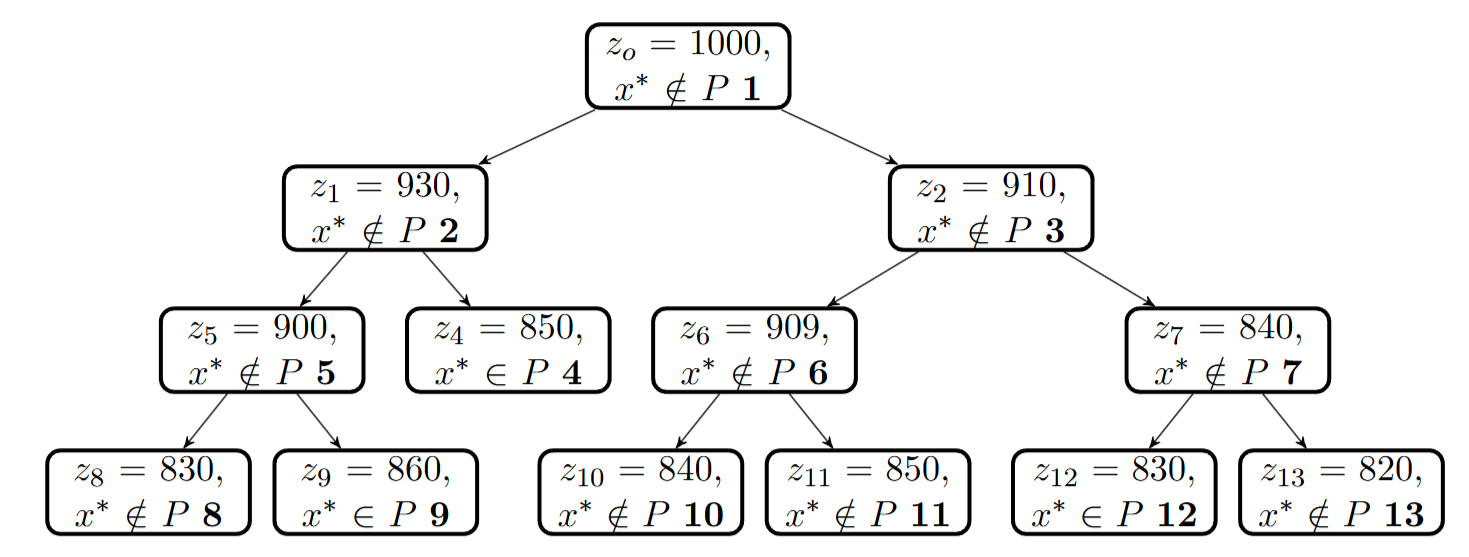
\includegraphics[width=1\linewidth]{img/ejercicios/Capitulo-5/ejercicio_5_1_arbol.png}
    \caption{Árbol de Branch and Bound}
    \label{ex:5:1:fig:arbol}
\end{figure}
